\chapter{I-Mode Pedestal Scalings}\label{ch:ImodePedestal}

The I-mode \cite{Whyte2010,Hubbard2011}, introduced in \cref{sec:hcr_imode}, is a novel high-performance regime pioneered on Alcator C-Mod.  I-mode is unique in that it appears to decouple energy and particle transport, forming a steep temperature pedestal with H-mode levels of energy confinement without the accompanying density pedestal or suppression of particle transport found in conventional H-modes.  I-mode exhibits several highly attractive properties for a putative reactor regime:

\begin{enumerate}
 \item Due to the lack of particle transport suppression (as is found in H-modes), the I-mode retains L-mode-like impurity confinement times, avoiding the accumulation of deleterious impurities in the plasma, including those from high-$Z$ metal plasma-facing components necessary for reactor operation \cite{Loarte2007}.  This ensures stationary operation without the need for ELMs or continuous fluctuations in the edge to provide the necessary relaxation of the particle confinement.
 \item I-mode appears to be naturally stable against large ELMs, avoiding excessive pulsed heat loading to plasma-facing components without externally-applied engineering controls (described in \cref{subsec:hcr_elmy_control}).
 \item Energy confinement in I-mode appears to exhibit little to know degradation with input heating power, in contrast to that found in ELMy H-mode ($\tau_E \sim P^{-0.7}$ from the ITER98y2 analysis \cite{ITER1999}), scaling quite favorably to reactor-scale devices.
\end{enumerate}

\begin{figure}[t]
 \pushtooutside
 \fcapside[60mm]{\caption[L-mode and I-mode edge profiles from a single discharge.]{L-mode (black) and I-mode (red) edge profiles from a single discharge.  I-mode maintains a comparable density profile (particularly, there is no change in $\nabla n_e$ or formation of a density pedestal), while forming an H-mode-like temperature pedestal.  \note{rescale, add detail?  repeat fig. 2.6?}}
 \label{fig:imode_pedestal}}{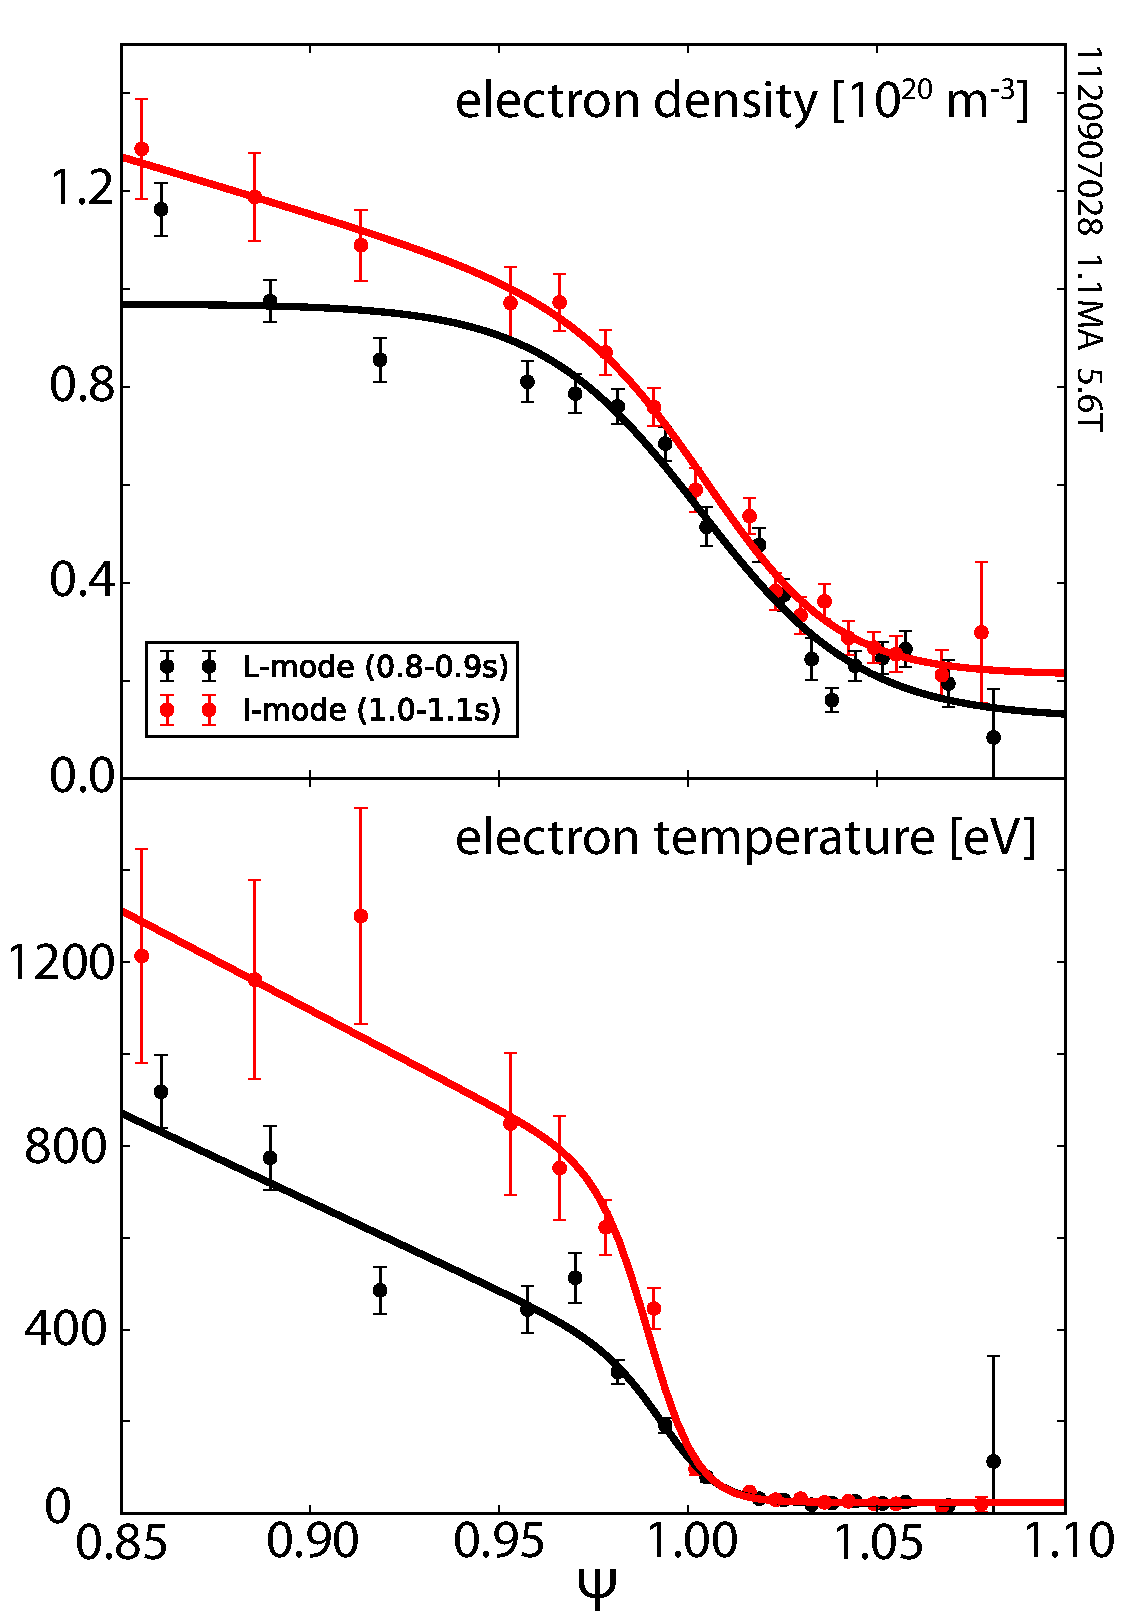
\includegraphics[width=100mm]{graphics/IModePedestal/1120907028_dens_temp.pdf}}
\end{figure}

A firm understanding of the pedestal is essential for the extrapolation of any high-performance regime to ITER- and reactor-scale devices.  The pedestal height sets a strong constraint on core temperature and pressure -- and therefore overall fusion performance -- both by acting as a boundary condition for the plasma profiles, and by supporting steeper core temperature gradients due to profile stiffness \cite{Kinsey2011,Hubbard1998}.  Moreover, the pedestal structure, particularly the steep gradients in density, temperature, and/or pressure, determines stability of the plasma against large, deleterious ELMs (see \cref{sec:mod_pb}).  In this chapter, we review empirical observations of the pedestal in I-mode from a recent series of dedicated experiments, with a focus on high-resolution pedestal profile measurements across a range of plasma parameters.  Through this, we examine trends in I-mode pedestal behavior, and their impact on global behavior and performance in I-mode, and possible extrapolations to larger devices\gnote{be more specific... maybe?}.\nicesectionending

\section{Access and Experimental Setup}\label{sec:imode_setup}

All data presented here was taken on the Alcator C-Mod tokamak, described in \cref{sec:intro_cmod}.  As described in \cref{subsec:hcr_imode_access}, I-mode access hinges primarily on operation with the ion $\nabla B$ drift (\cref{eq:gradbdrift}) directed away from the primary X-point in the plasma (the ``unfavorable $\nabla B$ drift'' configuration).  Within this requirement, though, I-mode access is fairly robust, with steady I-modes sustained in a variety of shapes -- both USN with standard field, and LSN shapes with reversed field to achieve the desired $\nabla B$ drift direction (in the latter case, the plasma current is reversed as well to preserve field helicity) -- and edge-current profiles, and at low-to-moderate collisionality (\cref{eq:nustar}).  The attainable range in $q_{95}$ and $\nu^*_{95}$ is shown in \cref{fig:imode_q_nustar}.  I-mode has been sustained with heating power up to $\sim 2 \times$ the L-I transition threshold power (see \cref{fig:imode_p_nebar_access}), above which the plasma typically enters an ELM-free H-mode (recall that operating with unfavorable $\nabla B$ drift elevates the H-mode threshold power by roughly a factor of two \cite{Suttrop2003,Carlstrom1998,Groebner1998}).

I-mode experiments in the most recent run campaigns have focused on reversed-field LSN plasmas, which exhibit the widest access window and avoid difficulties with power handling and edge diagnostics.  A subset of results from these experiments have been prepared with high-resolution pedestal measurements, optimized for analysis of the I-mode pedestal structure both from an empirical standpoint and for a computational approach to the pedestal stability; this data, herein termed the ``pedestal database'' (parameter range highlighted in \cref{fig:imode_q_nustar}) is stored in an SQL database (see \cref{app:sql}) for easy access and analysis, and will be used for the bulk of the I-mode work in this thesis (\cref{ch:ImodePedestal,ch:ImodeModeling}).

\begin{figure}[h]
 \pushtooutside
 \fcapside[60mm]{\caption[I-mode edge safety collisionality and safety factor.]{Range in edge collisionality $\nu^*_{95}$ and $q_{95}$ over which I-modes have been accessed.  Notably, I-mode operation is naturally favored near ITER targets for these parameters.  The subset of this data prepared with high-resolution pedestal profiles, herein termed the ``pedestal database'', is also highlighted.}\label{fig:imode_q_nustar}}{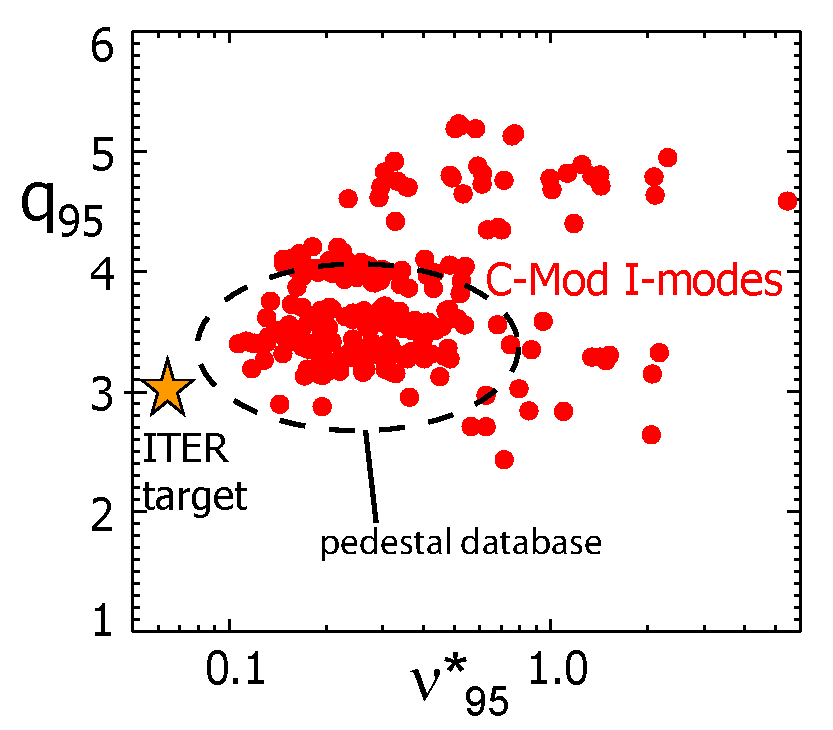
\includegraphics[width=100mm]{graphics/IModePedestal/q95_vs_nustar_2012_Imodeonly.pdf}}
\end{figure}

\begin{figure}[h]
 \pushtooutside
 \fcapside[60mm]{\caption[Density and power range for I-mode access]{Line-averaged density and loss power range for USN and LSN I-modes, illustrating $\sim 2 \times P_{L-I}$ range for $1-\SI{1.2}{\mega\ampere}$, $5-\SI{6}{\tesla}$ I-modes.  USN shapes are forward-field and LSN-shapes are reversed field, such that all I-modes shown are in the unfavorable drift configuration.  \note{swap for plot showing only high-res database, or merge?}}\label{fig:imode_p_nebar_access}}{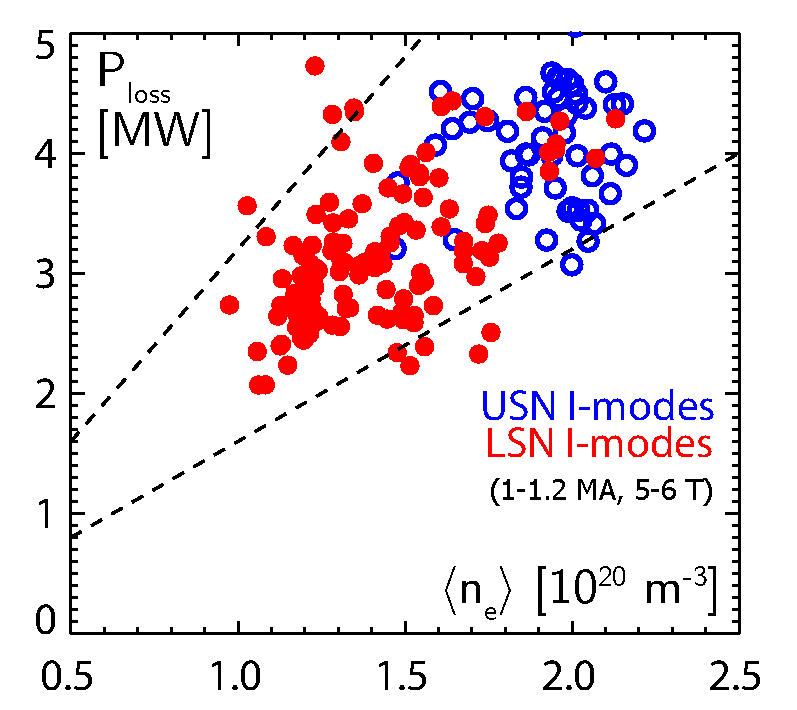
\includegraphics[width=100mm]{graphics/IModePedestal/Ploss_nebar_2013.pdf}}
\end{figure}

\nicesectionending

\section{Pedestal Responses}\label{sec:imode_height}

\noindent\note{introduce?}

\subsection{Pedestal Temperature}\label{subsec:imode_temp}

As the I-mode is characterized, in part, by its H-mode-like temperature pedestal and energy confinement, that is a suitable place to begin an examination of the I-mode pedestal.  A scan of plasma current from $\num{0.85}$ to $\SI{1.35}{\mega\ampere}$ reveals a positive trend of the pedestal temperature with plasma current, shown in \cref{fig:imode_Ip_Te95} with ELMy H-modes for comparison.  The I-mode temperature pedestal meets or exceeds the pedestal $T_e$ found in H-modes.  This is highly beneficial for global performance, as the high temperature pedestal coupled with stiff core temperature profiles supports very high (up to $\SI{8}{\kilo\electronvolt}$) core temperatures -- with moderately peaked core density profiles, this supports comparable core pressures and fusion reaction rates to H-mode despite the relaxed pedestal.\gnote{ref to plot?  ref neutron rates on C-Mod?}

There is, however, significant scatter at a given point in the $I_p$ scan, due to variation in the input heating power.  Examining a single current slice at $\SI{1.15}{\mega\ampere}$, shown in \cref{fig:imode_Pnebar_Te95}, we see a strong dependence of the temperature pedestal height on the net heating power, $P_{net} = P_{ICRF} + P_{Ohm} - P_{rad} - dW/dt$, normalized to (line-averaged) density -- effectively, the input power per particle.  A consistent pattern is observed at other current points.  The comparatively suppressed temperatures at the highest-current I-modes is a result of the higher fueling at these points, resulting in lower values of $P_{net}/\overline{n}_e$.

The temperature pedestal response in I-mode to plasma current is comparable to that seen in the density, temperature, and pressure pedestals in ELMy H-mode (\cf \cref{fig:elmy_ipscan}), although the sensitivity of the temperature pedestal in ELMy H-mode is somewhat weaker than in I-mode.  The response of the temperature pedestal to heating power is notable: the temperature in ELMy H-mode pedestals is only weakly dependent on power -- rather, increased heating power increases the ELM frequency and energy transport to maintain the approximately $\beta_p$-limited pedestal (\cf \cref{fig:hcr_elmybetas,fig:elmy_neBp_TeBp}).  Transport-limited EDA H-mode pedestals exhibit a similar trend \cite{Hubbard2001}, $T_{e,ped} \sim \left(P_{net}/\overline{n}_e\right)^{0.5 \pm 0.1}$, with the I-mode pedestal responding at least as strongly.  This behavior is quite desirable for a reactor scenario -- due to the strong response of the pedestal temperature to heating power, externally-applied heating power is an effective engineering control for core temperatures, and subsequently fusion reaction rates\gnote{move later, after discussing fueling?}.  

\begin{figure}
 \pushtooutside
 \fcapside[60mm]{\caption[Pedestal temperature vs. plasma current for I-mode and ELMy H-mode.]{Pedestal temperature versus plasma current for I-mode and ELMy H-mode.  I-mode temperature pedestals meet or exceed H-mode levels, and trend positively with current.  The spread in $T_{e,95}$ at a given current point is due to varying power per particle (see \cref{fig:imode_Pnebar_Te95}).  The highest-current I-modes exhibit temperatures below the bulk trend due to low values of $P_{net}/\overline{n}_e$, as these I-modes were fueled to comparatively high densities.}\label{fig:imode_Ip_Te95}}{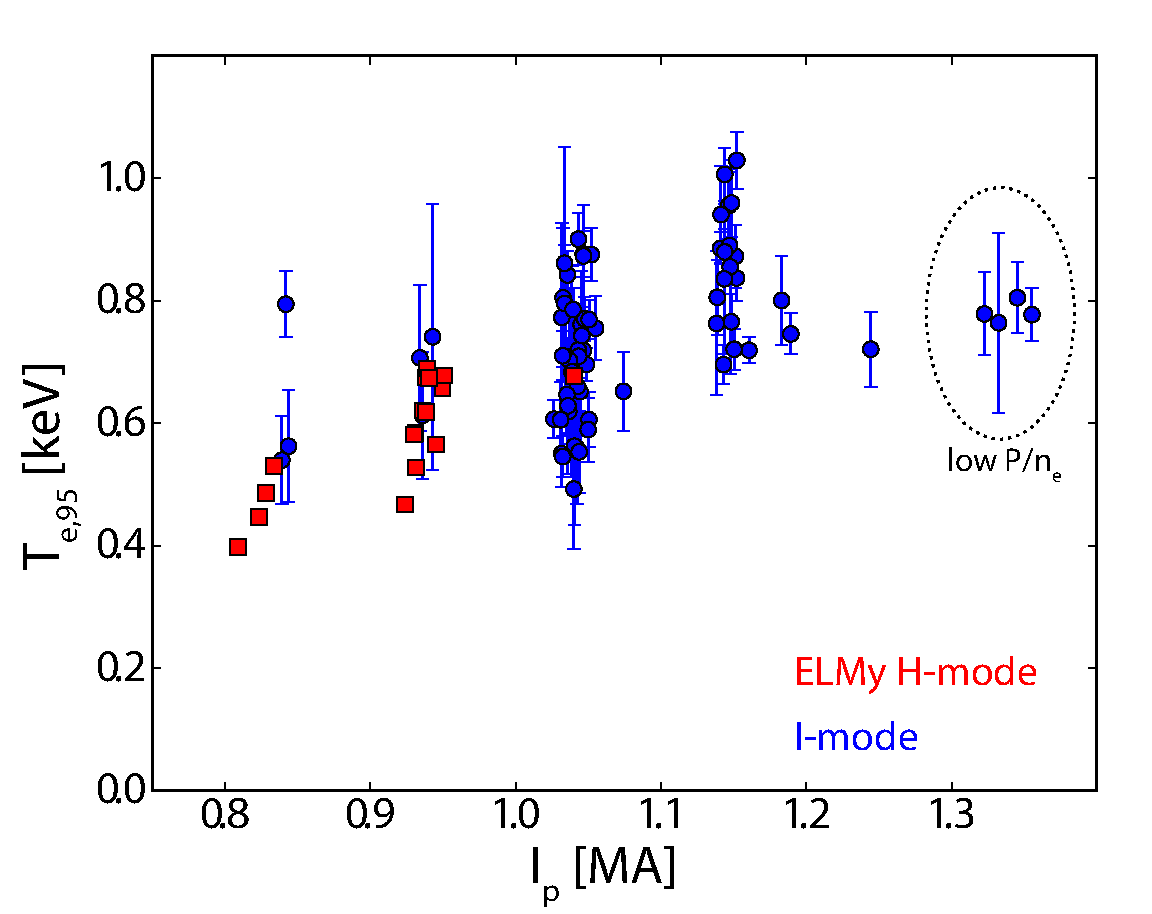
\includegraphics[width=100mm]{graphics/IModePedestal/Ip_Te95.pdf}}
\end{figure}

\begin{figure}
 \pushtooutside
 \fcapside[60mm]{\caption[Pedestal temperature vs. heating power per particle for an example current slice.]{Pedestal temperature $T_{e,95}$ vs. heating power per particle ($P_{net}/\overline{n}_e$) for the $\SI{1.15}{\mega\ampere}$ current slice, illustrating the approximately-linear trend in temperature at fixed current.  This behavior is highly beneficial as an external control for the pedestal temperature.}\label{fig:imode_Pnebar_Te95}}{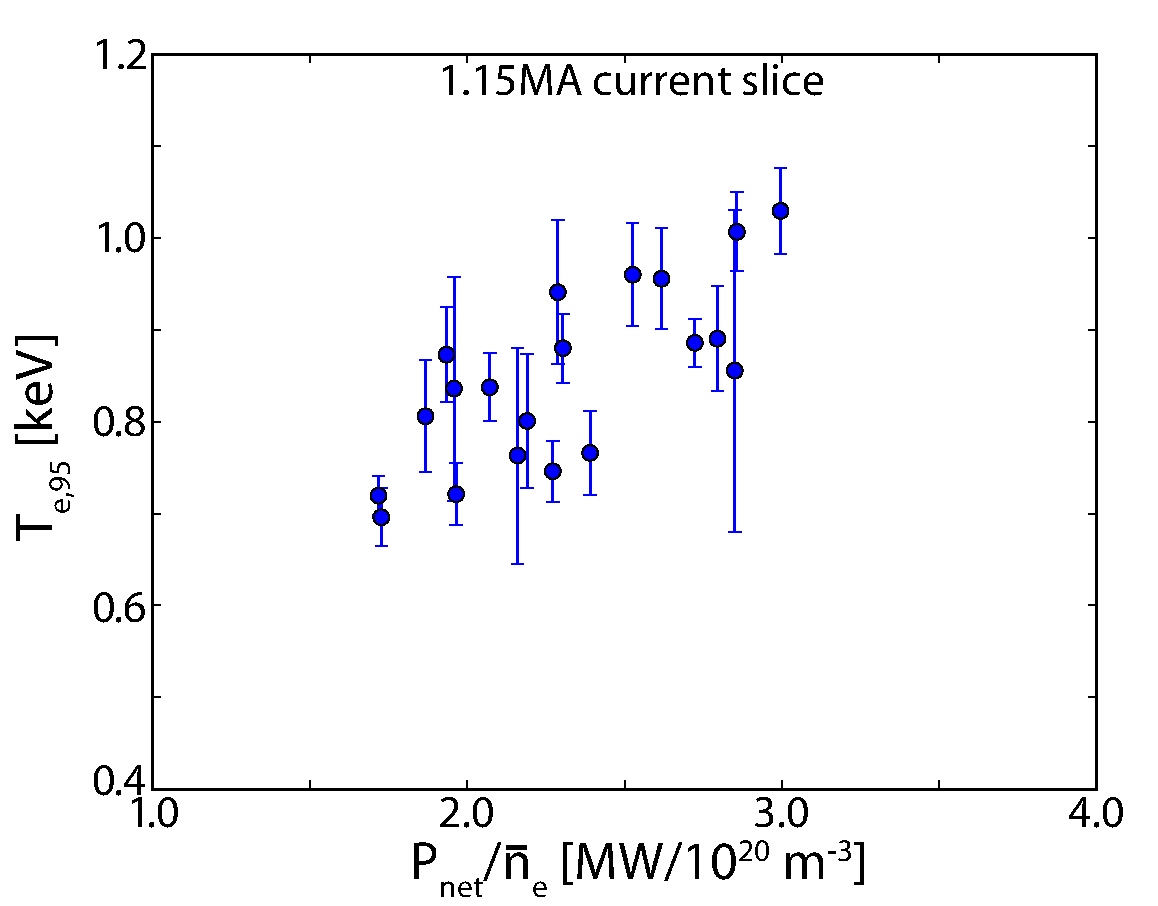
\includegraphics[width=100mm]{graphics/IModePedestal/Pnebar_Te95_115MA.pdf}}
\end{figure}

\subsection{Pedestal Response to Fueling}\label{subsec:imode_fueling}

In contrast to the temperature pedestal (\cref{subsec:imode_temp}), the edge density in I-mode exhibits markedly different behavior compared to conventional H-modes.  Edge density is set primarily through operator fueling control via gas puffing, maintaining an L-mode-like density profile without the density pedestal found in H-mode.\gnote{mention neutral opacity in C-Mod, prospects for edge gas fueling?}  Given sufficient heating power, temperature pedestals can be maintained with increased density due to the strong response of $T_{e,95}$ to power-per-particle.  Example discharges matched in current, field, and shaping are shown in \cref{fig:imode_fuelingprofiles}, spanning a range in fueling and heating power, $\overline{n}_e = 1.0 - \SI{1.7e20}{\per\meter\cubed}$, $P_{net} = 2.75 - \SI{4.10}{\mega\watt}$.  Temperature pedestals are matched across all three discharges, using consistent power-per-particle $P_{net}/\overline{n}_e = 2.4 - \SI{2.7}{\mega\watt}/10^{20}\;\si{\per\meter\cubed}$.\gnote{note edge vs integrated density, L-mode-like profile?}

This behavior is distinct from that found in H-modes on C-Mod.  ELMy H-modes at fixed current and shaping exhibit an inverse relationship between pedestal $n_e$ and $T_e$ due to limited pedestal $\beta_p$, such that increased fueling tends to cool the pedestal (although the modification of pedestal collisionality also modifies the ELM character\gnote{find cite}).  EDA H-modes lack the fueling control found in I-mode, instead railing the pedestal density to a value set by the plasma current, such that the outward transport and strong inward particle pinch are balanced.  This is indicative of a path to strongly improved performance in I-mode, increasing pedestal $\beta_p$ and global confinement via matched increases in fueling and heating power, maintaining the target temperature pedestal with appropriate levels of $P_{net}/\overline{n}_e$.  Recent experiments on C-Mod \cite{Hubbard2012} have successfully applied this approach, reaching elevated density by fueling into an established I-mode despite the application of heating power levels sufficient for a transition to H-mode at a higher starting density.\gnote{plans for ITER}

\begin{figure}[ht]
 \pushtooutside
 \fcapside[60mm]{\caption[Density and temperature pedestals at matched current and field with varying fueling and heating power -- matched $P_{net}/\overline{n}_e$ maintains the $T_e$ pedestal.]{Density and temperature pedestals at matched current, field, and shaping, with varying fueling and heating power levels.  The three discharges are fueled to $\overline{n}_e$ of $\num{1.0}$ (black), $\num{1.3}$ (blue), and $\SI{1.7e20}{\per\meter\cubed}$ (red) respectively, with heating powers of $\num{2.75}$, $\num{3.65}$, and $\SI{4.10}{\mega\watt}$ to maintain matched $P_{net}/\overline{n}_e \sim 2.4-2.7$.  The constant power-per-particle maintains matched temperature pedestals across the fueling range, indicative of the independent control of pedestal $n_e$ and $T_e$ available in I-mode.}\label{fig:imode_fuelingprofiles}}{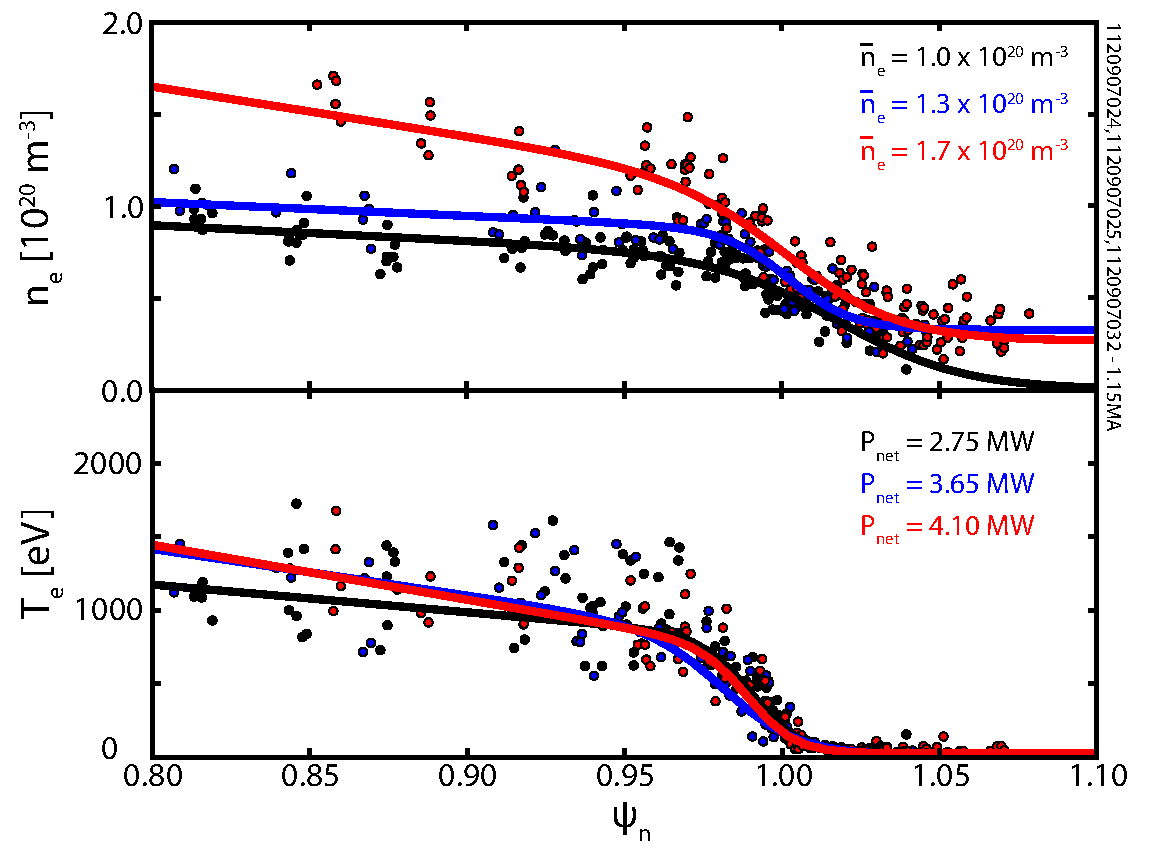
\includegraphics[width=100mm]{graphics/IModePedestal/fuelingprofiles.pdf}}
\end{figure}

\subsection{Pressure Pedestal Scalings and Performance}\label{subsec:imode_pres}

Despite lacking a density pedestal, I-mode is capable of reaching competitive levels of pedestal thermal pressure, while maintaining favorable behavior  in its particle (particularly impurities -- see \cref{fig:hcr_imode_taui}) transport and temperature pedestal.  I-mode pedestal pressure (we use twice the electron pressure from Thomson Scattering here, consistent with $T_i \approx T_e$ measurements in well-equilibrated pedestals on C-Mod \cite{Hubbard2011} and with the relatively low impurity contribution to the pressure, $Z_{eff} \sim 2$) versus plasma current is shown in \cref{fig:imode_Ip_p95}, with additional differentiation by fueling level indicated by color.  An increase in pedestal pressure by at least $p_{95} \sim I_p$ is observed, consistent with the scaling of the temperature pedestal $T_e \sim I_p$.  The pedestal pressure at a given current is seen to increase strongly with increased fueling, consistent with the maintenance of the temperature pedestal with increased heating power and matched fueling (and thus constant levels of $P_{net}/\overline{n}_e$).

The effect of heating power on the pressure pedestal is visible in \cref{fig:imode_Pnet_p95}, showing the $\SI{1.15}{\mega\ampere}$ current slice (see \cref{fig:imode_Pnebar_Te95} for the same).  At fixed current, the pressure pedestal scales as $p_{95} \sim P_{net}$, consistent with the previously observed $T_{e,95} \sim P_{net}/\overline{n}_e$ trend in the temperature pedestal as $p_{95} \sim n_{e,95} T_{e,95}$\gnote{$n_{e,95} \sim \overline{n}_e$}.  This is consistent with the favorable scaling of energy confinement in I-mode with heating power -- plasma stored energy is set by heating power and the energy confinement time, $W \sim P \tau_E$, and is strongly influenced by the pedestal pressure\gnote{cite?}.  Thus, the trend $p_{95} \sim P_{net}$ is consistent with little or no degradation of $\tau_E$ with heating power, which has been observed in global measurements of I-mode \cite{Dominguez2012,Whyte2010}, and is distinct from the trend $\tau_E \sim P^{-0.7}$ found for ELMy H-modes \cite{ITER1999}.  This behavior is quite favorable when scaled to large, high-power machines, particularly when an appreciable level of fusion self-heating is projected\gnote{reword}.

Trends in the pressure pedestal in I-mode are also indicative of MHD stability.  As shown in \cref{fig:imode_ip_gradp}, the peak pressure gradient (identified as the driver for ballooning MHD instabilities, described in \cref{subsec:mod_balloon}, and the trigger for large ELMs\gnote{cite?}) in I-mode is consistently shallower at a given $I_p$ than comparable ELMy H-modes on C-Mod, due to the flat edge density profile.  Moreover, the pedestal pressure gradient scales more weakly than the expected $\nabla p \sim I_p^2$ expected from the ballooning stability boundary \cite{Connor1978}.  The intuitive conclusion from this is that I-mode is generally stable to the MHD instabilities identified with the ELM trigger -- the MHD stability and ELM behavior of I-mode is explored in detail in \cref{ch:ImodeModeling}.

\begin{figure}
 \pushtooutside
 \fcapside[60mm]{\caption[Pedestal pressure versus plasma current in I-mode and ELMy H-mode.]{Pedestal thermal pressure ($2 \times p_{e,95}$) versus plasma current, colored by fueling level indicated by line-averaged density $\overline{n}_e$.  The shaded region indicates the typical range of pedestal pressures in C-Mod ELMy H-modes.  A strong, roughly $p_{95} \sim I_p$ trend in pedestal pressure is observed.  At a given current, a sstrong increase in pedestal pressure with fueling is also observed (note: heating power also varied in these discharges).}\label{fig:imode_Ip_p95}}{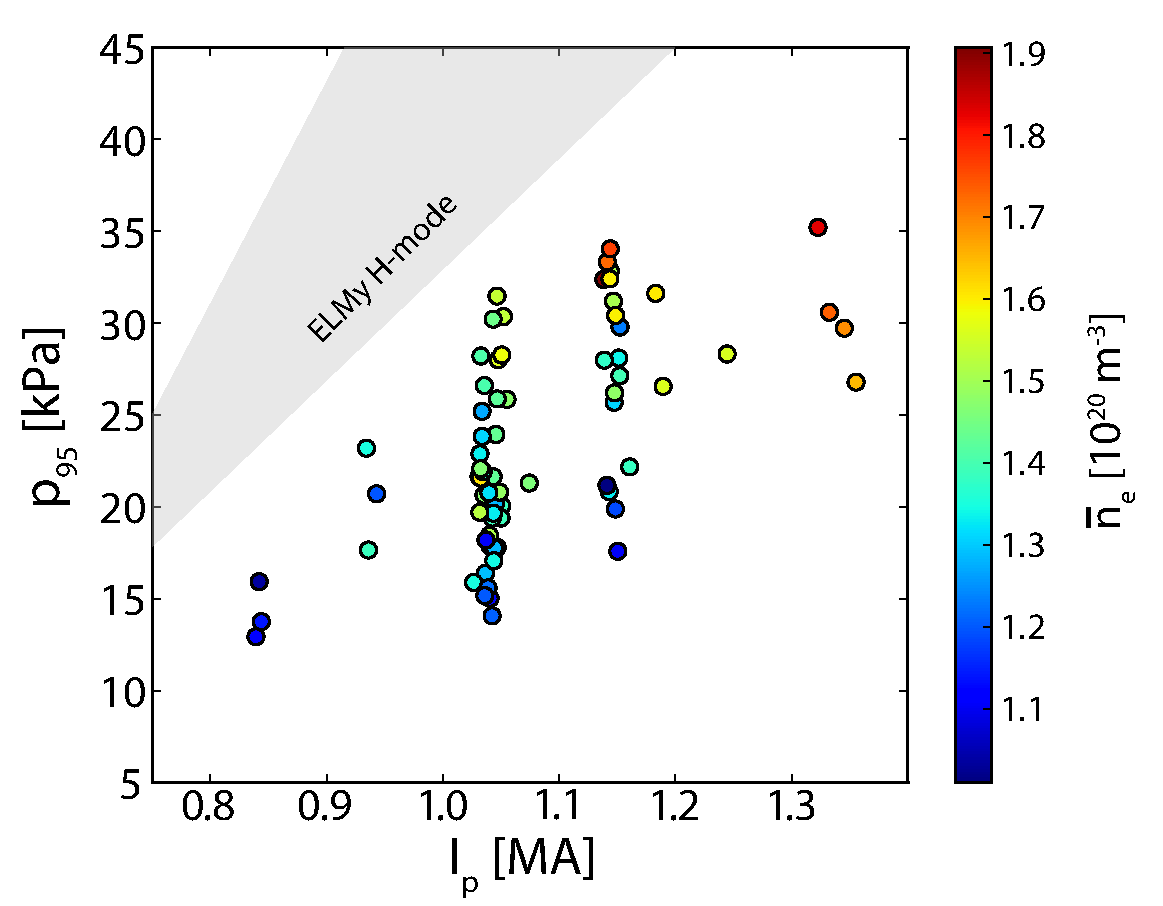
\includegraphics[width=100mm]{graphics/IModePedestal/Ip_p95_nebar.pdf}}
\end{figure}

\begin{figure}
 \pushtooutside
 \fcapside[60mm]{\caption[Pedestal pressure vs. heating power for an example current slice.]{Pedestal pressure ($2\times p_{e,95}$) versus net heating power for the $\SI{1.15}{\mega\ampere}$ current slice, illustrating the trend $p_{95} \sim P_{net}$ at fixed current.  This is consistent with the power trend in the I-mode temperature pedestal, $T_{e,95} \sim P_{net}/\overline{n}_e$.}\label{fig:imode_Pnet_p95}}{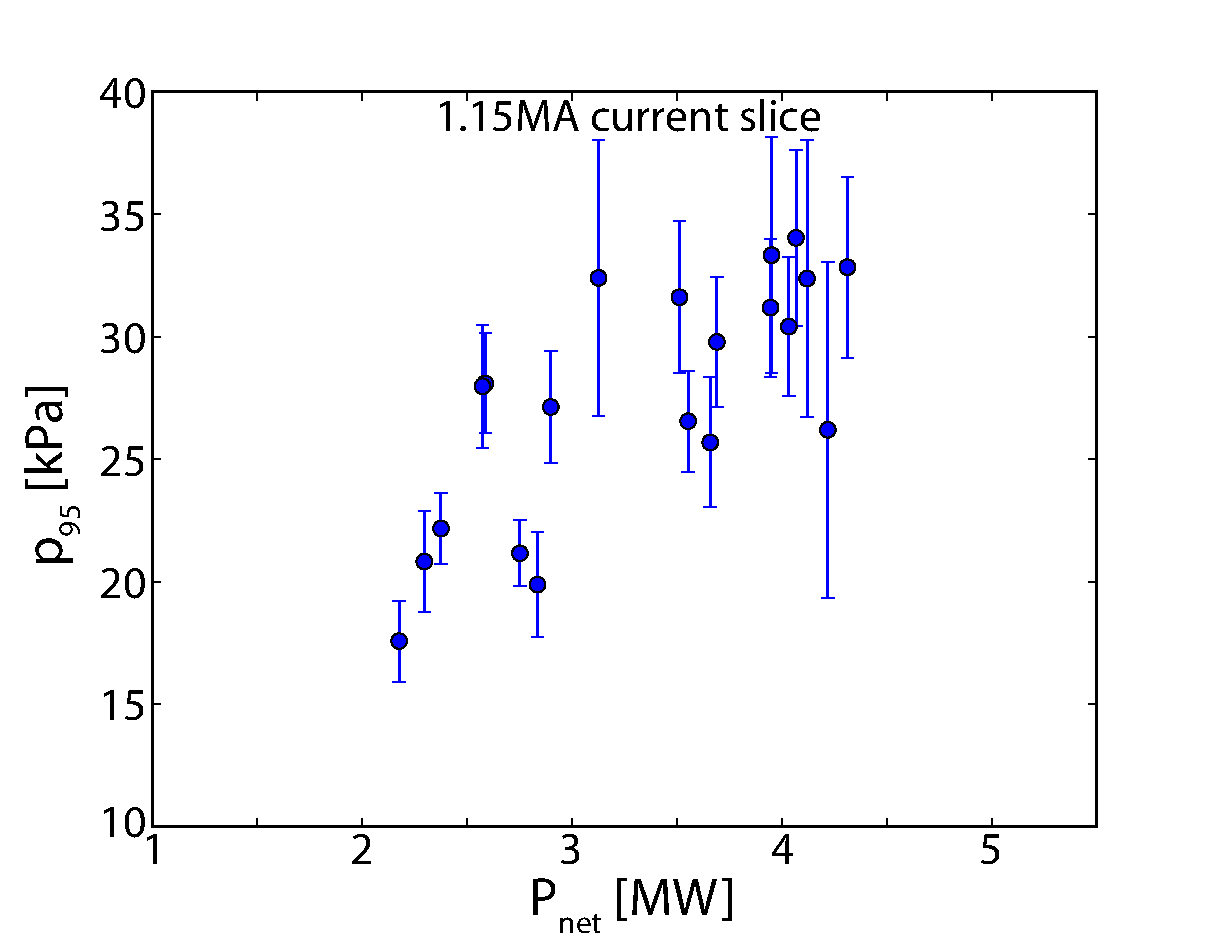
\includegraphics[width=100mm]{graphics/IModePedestal/Pnet_p95_115MA.pdf}}
\end{figure}

\begin{figure}
 \pushtooutside
 \fcapside[60mm]{\caption[Pressure gradient vs. plasma current for I-mode and ELMy H-mode.]{Peak pressure gradient (measured at the pedestal midpoint) versus plasma current for I-mode and ELMy H-mode.  I-mode consistently exhibits a weaker pressure gradient at a given current, as well as scaling more weakly than the $\nabla p \sim I_p^2$ expected from the ballooning MHD stability limits associated with ELMy H-mode.}\label{fig:imode_ip_gradp}}{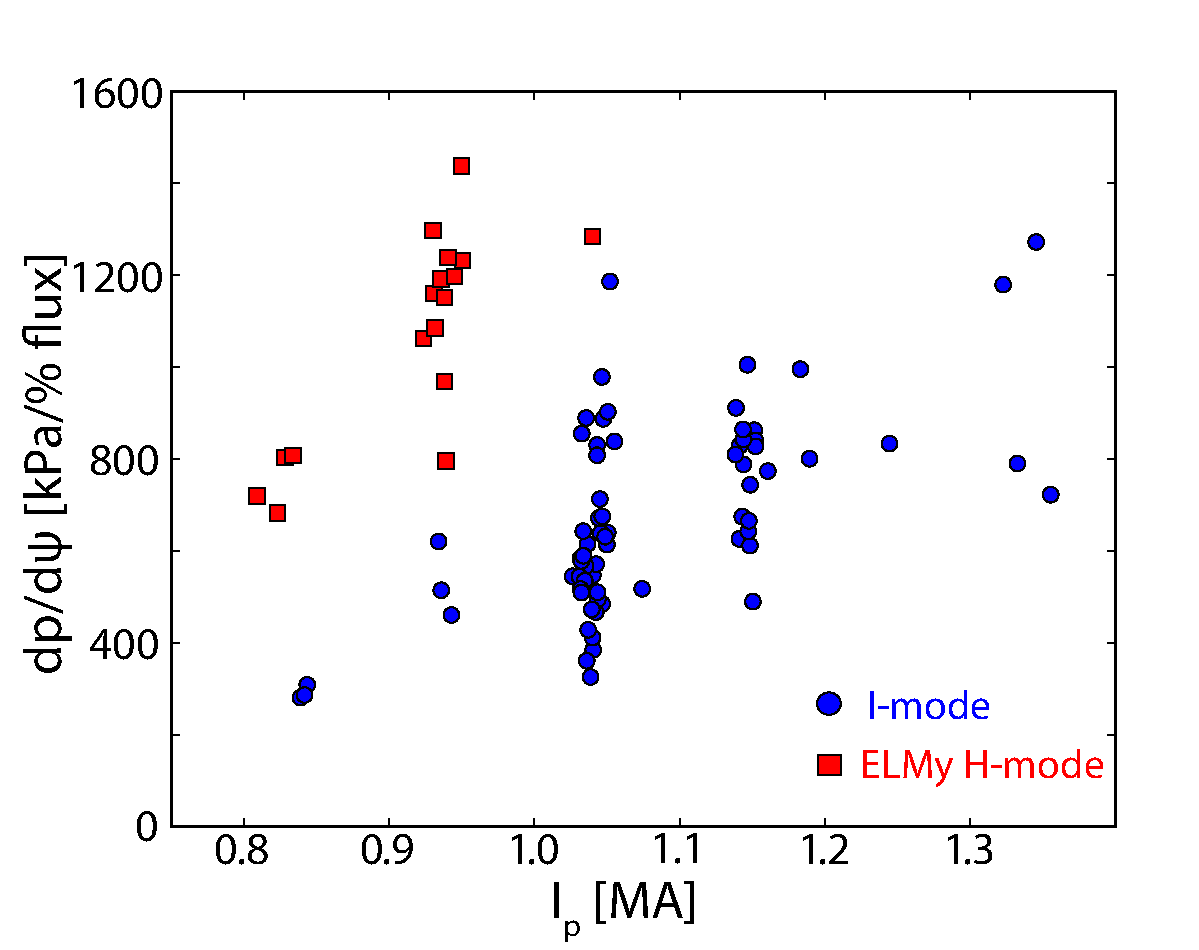
\includegraphics[width=100mm]{graphics/IModePedestal/Ip_gradp.pdf}}
\end{figure}

\nicesectionending

\section{Pedestal Widths}\label{sec:imode_width}

\begin{figure}
 \pushtooutside
 \fcapside[60mm]{\caption[Pedestal width vs. poloidal beta in I-mode and ELMy H-mode.]{Pedestal width versus poloidal beta in I-mode and ELMy H-mode.  ELMy H-modes lie on the $\Delta_\psi \sim \beta_{p,ped}^{1/2}$ line predicted for KBM-limited pedestals (see \cref{subsec:elmy_eped_width}).  I-mode shows no scaling of the pedestal width with $\beta_p$, and exhibits pedestals consistently wider than predicted for comparable ELM-limited pedestals.}\label{fig:imode_wid_betapol}}{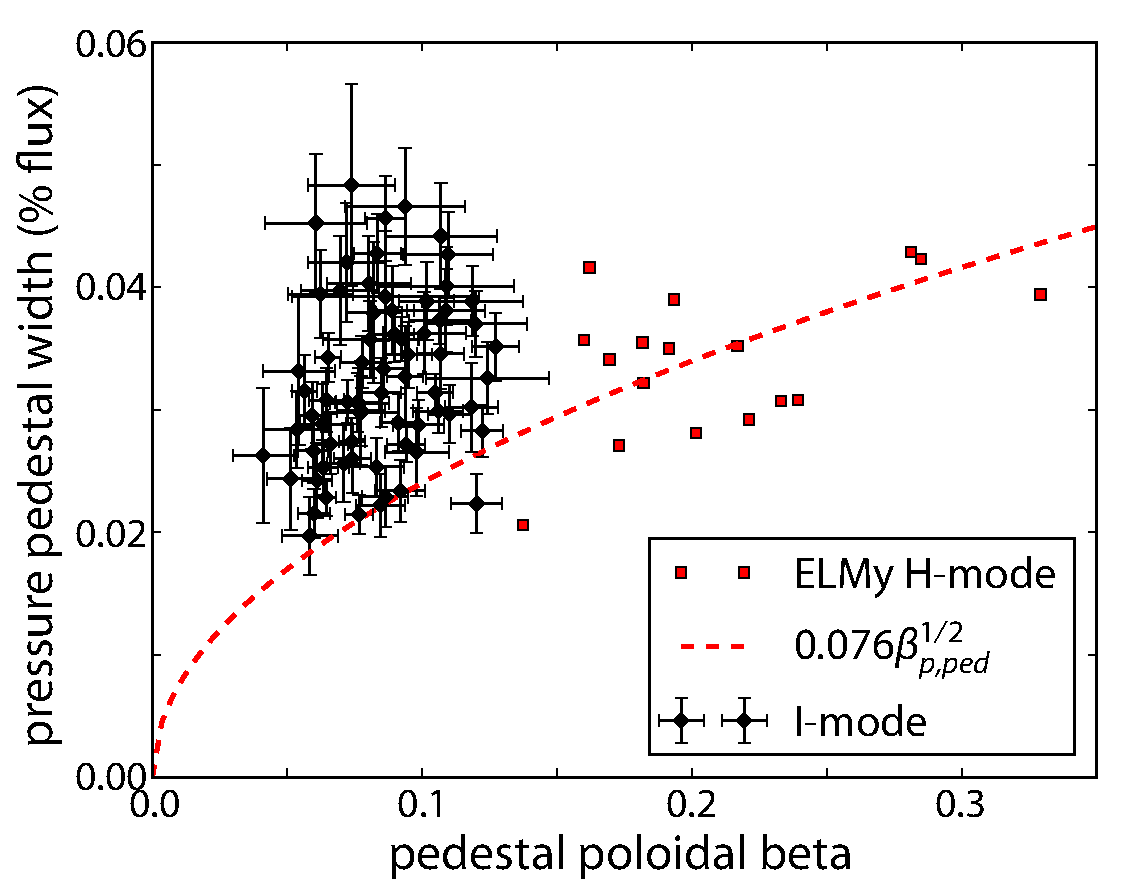
\includegraphics[width=100mm]{graphics/IModePedestal/wid_betapol.pdf}}
\end{figure}

\nicesectionending

\section{Global Behavior, Performance, \& Confinement}\label{sec:imode_confinement}

\begin{figure}
 \pushtooutside
 \fcapside[60mm]{\caption[]{}\label{fig:imode_coreprofs}}{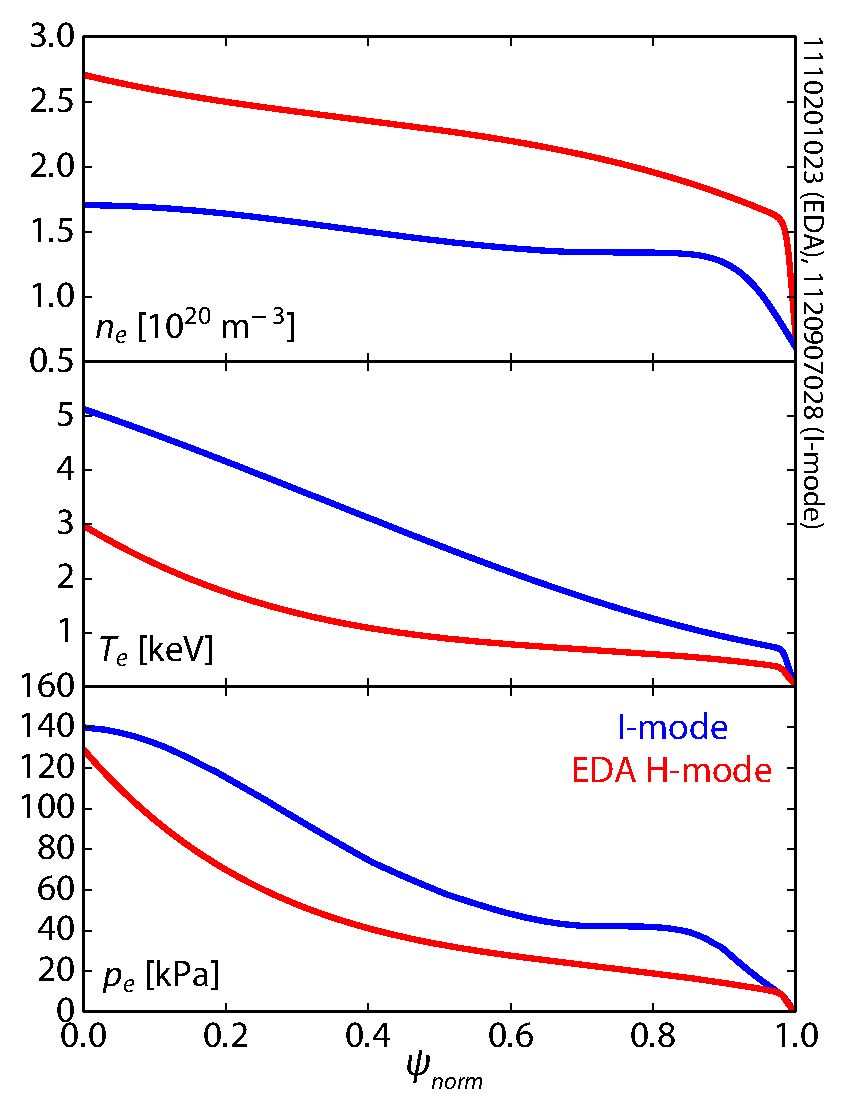
\includegraphics[width=100mm]{graphics/IModePedestal/coreprof.pdf}}
\end{figure}

\begin{figure}
 \pushtooutside
 \fcapside[60mm]{\caption[]{}\label{fig:imode_PIp_W}}{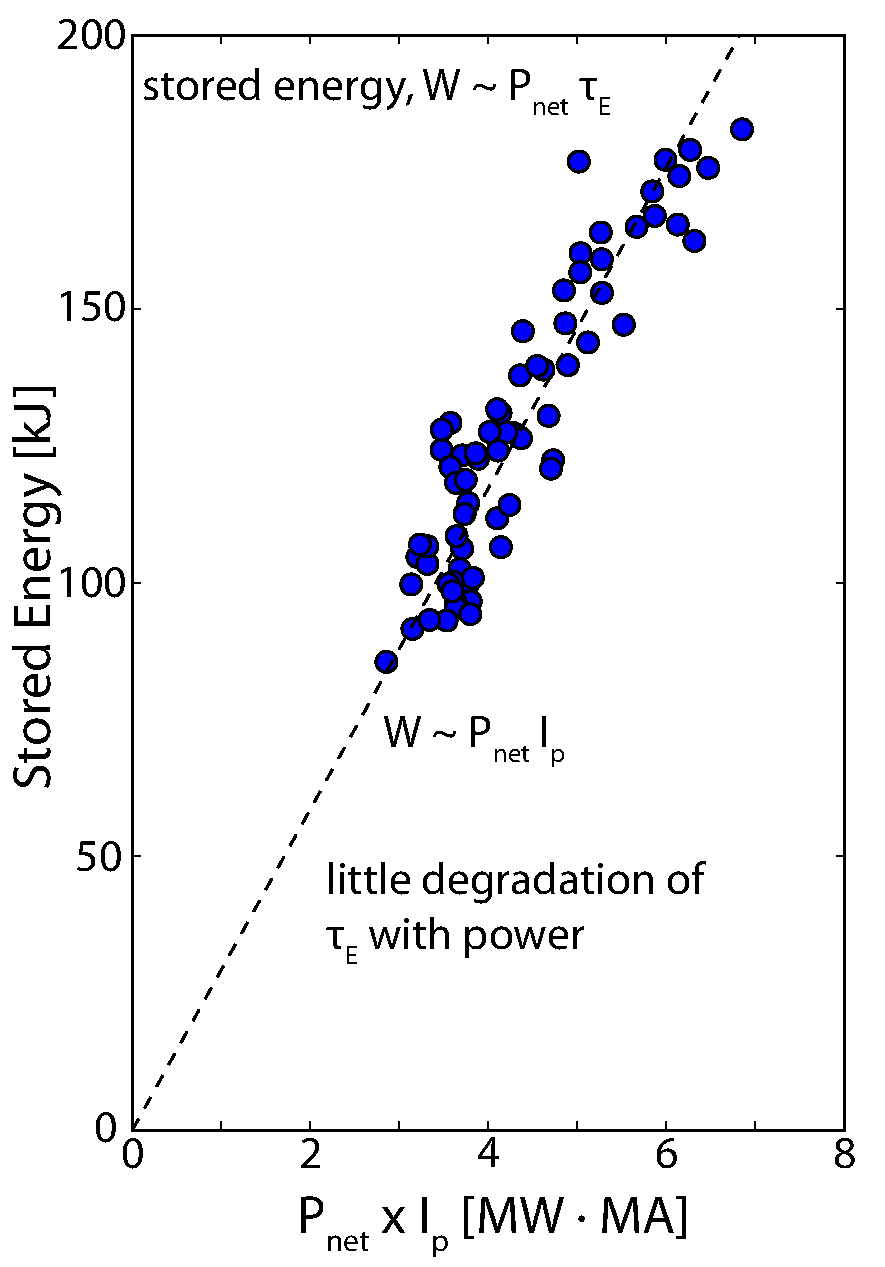
\includegraphics[width=100mm]{graphics/IModePedestal/PIp_W_scale.pdf}}
\end{figure}

\subsection{Confinement Scaling Laws}\label{subsec:imode_powerlaws}

Due to the complexity inherent in modeling global energy transport from first-principles physics, it is common to establish empirical scaling laws for energy confinement using a power-law fit to large datasets.  For example, the ITER89 \cite{Yushmanov1990} and ITER98 \cite{ITER1999} scalings utilized an extensive multi-machine database \cite{Christiansen1992} for L-mode and H-mode confinement.  In particular the ITER98y2 scaling (see \cref{eq:tau98}) is a commonly-used baseline for high-performance regimes, particularly in terms of the normalized $H_{98}$ (\cref{eq:H98}).  However, as the ITER98y2 scaling was constructed predominantly with type-I ELMy H-modes (as these customarily are the highest-performance H-modes on most tokamaks), and as such implicitly includes the physics of ELM-limited pedestals.  For example, the power-law fit in ITER98y2 includes a strong degradation of confinement with heating power, $\tau_E \sim P^{-0.7}$.  This is consistent with the observed weak response of ELMing pedestals with heating power \cite{Snyder2007}, with increased power instead raising the ELM frequency to maintain consistent ELM-driven heat transport.\gnote{cite}

In light of the substantially different physics of the I-mode pedestal and energy confinement compared to H-modes\gnote{clarify}, it is useful to construct a power-law confinement fit using I-mode data.  It is strongly emphasized that such a fit would be only preliminary, as fits using data from a single machine lack the range of parameter values needed to fully constrain the fit.  Even so, it is illustrative to examine the results of I-mode under an analogous approach, indicative of the potential benefits of I-mode operation when extrapolated to larger devices.\gnote{reword}  I-mode energy confinement times are fitted in a least-squares sense to the general form

\begin{equation}\label{eq:taufit}
 \tau_{I-mode} = C \; I_p^{\alpha_{I_p}} \; B_T^{\alpha_{B_T}} \; \overline{n}_e^{\alpha_{n_e}} \; R^{\alpha_R} \; \varepsilon^{\alpha_\varepsilon} \; \kappa^{\alpha_\kappa} \; P_{loss}^{\alpha_P}
\end{equation}

\noindent to find free exponents $\alpha_j$ for plasma current $I_p$ in $\si{\mega\ampere}$, toroidal field $B_T$ in $\si{\tesla}$, line-averaged density $\overline{n}_e$ in $\SI{e20}{\per\meter\cubed}$, major radius $R$ in $\si{\meter}$, inverse aspect ratio $\varepsilon$, elongation $\kappa$, and loss power $P_{loss}$ in $\si{\mega\watt}$ (see \cref{eq:ploss}).  To extend the quantity of data and range of parameters available for this assay, the high-resolution pedestal data used in the bulk of this thesis is supplemented by older I-mode datasets containing both reversed-field LSN and forward-field USN I-mode cases.  Although these data lack the high-resolution edge data necessary for pedestal structure and stability studies, they are nevertheless suitable for scalings based on global parameters.  Although the net power $P_{net}$ (see \cref{eq:pnet}) has been demonstrated to be the more accurate parameter, rather than $P_{loss}$\gnote{cite, clarify}, these older data contain inconsistent measurements of the radiated power, necessitating the use of loss power in its stead (and in any case, this is consistent with previous confinement scaling studies).

Results from a number of scaling studies are shown in \cref{tab:imode_confinement}, containing the values and standard deviations for each exponent value, the scale factor $C$, and the $R^2$ coefficient of determination.  We begin with the full parameter list used in the ITER98y2 scaling, shown as fit \#1 in \cref{tab:imode_confinement}, with results shown in \cref{fig:imode_tauE_1}.  However, it is immediately obvious that the size scalings, dependent on major radius $R$ and inverse aspect ratio $\varepsilon$, are not properly captured (denoted by the extreme errorbars on these parameters).  This is to be expected -- absent meaningful variation in $R$ and $\varepsilon$ in the dataset (which requires multiple machines to produce) these parameters are not well-constrained, and result \#1 is over-fitted.  For simplicity, we reduce our consideration to an effective single-machine scaling, omitting these parameters (indicated by blank entries in \cref{tab:imode_confinement}).  

\begin{table*}
 \pushtooutside
 \ttabbox{\caption[Parameters for power-law scalings of I-mode energy confinement time.]{Parameters for power-law scalings of the I-mode energy confinement time $\tau_E$, along with $R^2$ coefficients of determination for the fit.  Blank entries indicate parameters that were omitted from that fit.  Note that fit \#5 utilized a fixed $R^2 \sqrt{\varepsilon}$ size dependence rather than taking the size to be a free fitting parameter.  Parameters are in the given units: $I_p$ in $\si{\mega\ampere}$, $B_T$ in $\si{\tesla}$, $\overline{n}_e$ in $\SI{e20}{\per\meter\cubed}$, $R$ in $\si{\meter}$, and $P_{loss}$ in $\si{\mega\watt}$.  Elongation $\kappa$ and aspect ratio $\varepsilon$ are dimensionless.}\label{tab:imode_confinement}}{
 \begin{tabular}{cccccc}
  \toprule
  & \#1 & \#2 & \#3 & \#4 & \#5 \\
  \midrule
  $C$ & $0.040 \pm 0.066$ & $0.007 \pm 0.002$ & $0.014 \pm 0.002$ & $0.014 \pm 0.002$ & $0.056 \pm 0.008$ \\
  $I_p$ & $0.686 \pm 0.074$ & $0.696 \pm 0.073$ & $0.685 \pm 0.076$ & $0.692 \pm 0.073$ & $0.676 \pm 0.077$ \\
  $B_T$ & $0.698 \pm 0.075$ & $0.697 \pm 0.071$ & $0.768 \pm 0.072$ & $0.773 \pm 0.071$ & $0.767 \pm 0.072$ \\
  $\overline{n}_e$ & $-0.077 \pm 0.055$ & $-0.050 \pm 0.048$ & $0.017 \pm 0.048$ & & $0.006 \pm 0.048$ \\
  $R$ & $4.219 \pm 4.623$ & & & & $2^*$ \\
  $\varepsilon$ & $0.127 \pm 1.144$ & & & & $0.5^*$ \\
  $\kappa$ & $1.686 \pm 0.398$ & $1.501 \pm 0.350$ & & & \\
  $P_{loss}$ & $-0.197 \pm 0.048$ & $-0.220 \pm 0.043$ & $-0.286 \pm 0.042$ & $-0.281 \pm 0.039$ & $-0.275 \pm 0.042$ \\
  $R^2$ & $0.713$ & $0.711$ & $0.685$ & $0.684$ & $0.683$ \\
  \bottomrule
 \end{tabular}
 }
\end{table*}

\begin{figure}
 \pushtooutside
 \fcapside[60mm]{\caption[Power-law fit to I-mode $\tau_E$ with full parameter set.]{Power-law fit for I-mode energy confinement time $\tau_E$, fitted using the full ITER98y2 parameter set (fit \#1 in \cref{tab:imode_confinement}).  Both the high-resolution pedestal database and older reversed-field LSN and forward-field USN I-mode databases are used.  While the fit is generally good, lack of variation in certain parameters -- particularly the size parameters $R$ and $\varepsilon$ (as expected for a single-machine scaling), and elongation $\kappa$ mean that the true variation with these parameters is not accurately captured.  However, the expected weak degradation of $\tau_E$ with heating power is captured.}\label{fig:imode_tauE_1}}{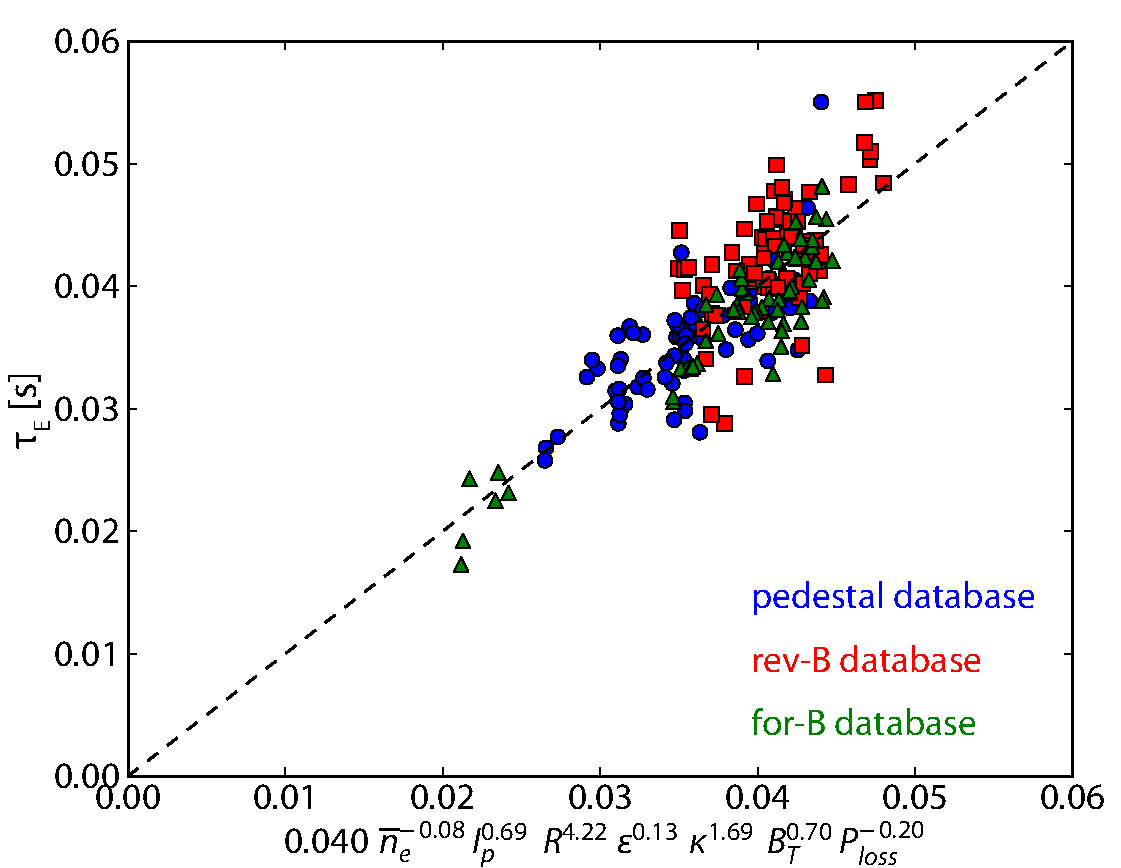
\includegraphics[width=100mm]{graphics/IModePedestal/tauE_1_Ploss_sep.pdf}}
\end{figure}

\begin{figure}
 \pushtooutside
 \fcapside[60mm]{\caption[Power-law fit to I-mode $\tau_E$, with poorly-fitted parameters excluded.]{Power-law fit for I-mode energy confinement time $\tau_E$, fitted with the size parameters $R$ and $\varepsilon$, and elongation $\kappa$ excluded due to the lack of variation in these variables in the available data (fit \#3 in \cref{tab:imode_confinement}).  Both the high-resolution pedestal database and older reversed-field LSN and forward-field USN I-mode databases are used.}\label{fig:imode_tauE_3}}{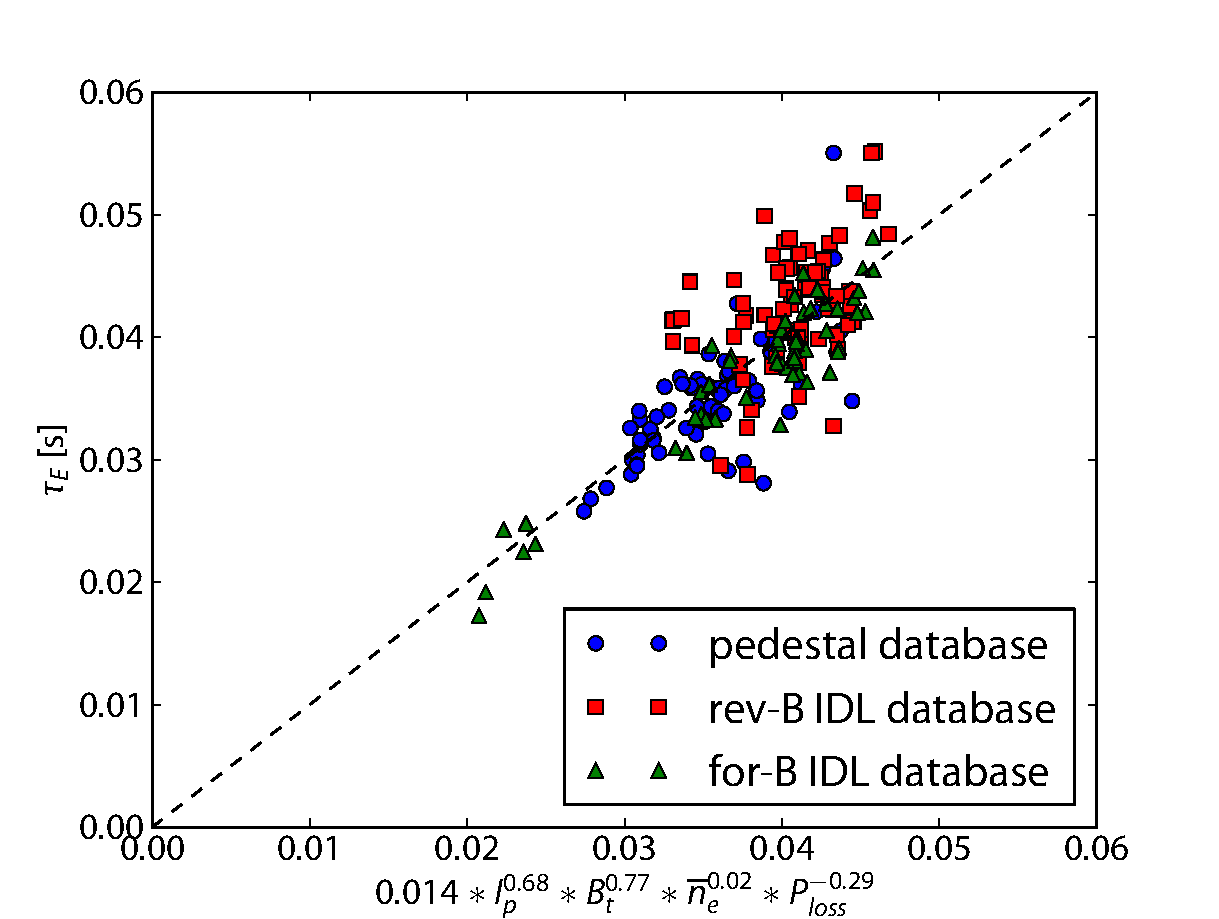
\includegraphics[width=100mm]{graphics/IModePedestal/tauE_3_Ploss_sep.pdf}}
\end{figure}

\begin{figure}
 \pushtooutside
 \fcapside[60mm]{\caption[Power-law fit to I-mode $\tau_E$, with fixed $R^2 \sqrt{\varepsilon}$ size scaling.]{Power-law fit to I-mode energy confinement time $\tau_E$, with the \emph{ansatz} of an $R^2 \sqrt{\varepsilon}$ size scaling fixed (fit \#5 in \cref{tab:imode_confinement}).  Both the high-resolution pedestal database and older reversed-field LSN and forward-field USN I-mode databases are used.  Note the expected weak degradation of $\tau_E$ with heating power.}\label{fig:imode_tauE_6}}{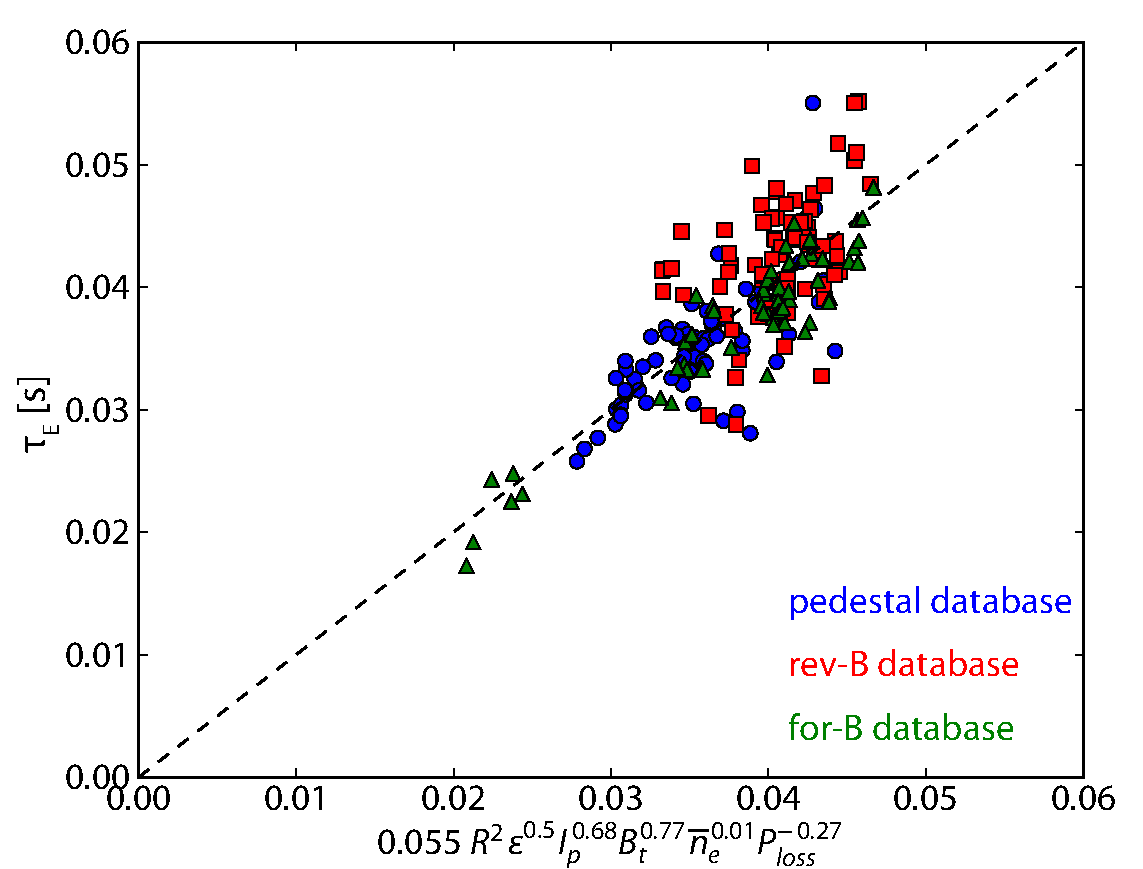
\includegraphics[width=100mm]{graphics/IModePedestal/tauE_6_Ploss_sep.pdf}}
\end{figure}

\begin{figure}
 \pushtooutside
 \fcapside[60mm]{\caption[Power-law fit to I-mode $\tau_E$ extrapolated to larger devices.]{Modeled energy confinement time $\tau_E$ with the fixed $R^2 \sqrt{\varepsilon}$ size scaling (fit \#5 in \cref{tab:imode_confinement}, extrapolated to DIII-D, ASDEX Upgrade, JET, and ITER.  Modeled energy confinement times are competitive with H-modes, both the measured $\tau_E$ for existing machines and the expected ITER98y2 prediction for ITER H-modes.}\label{fig:imode_tauE_extrap}}{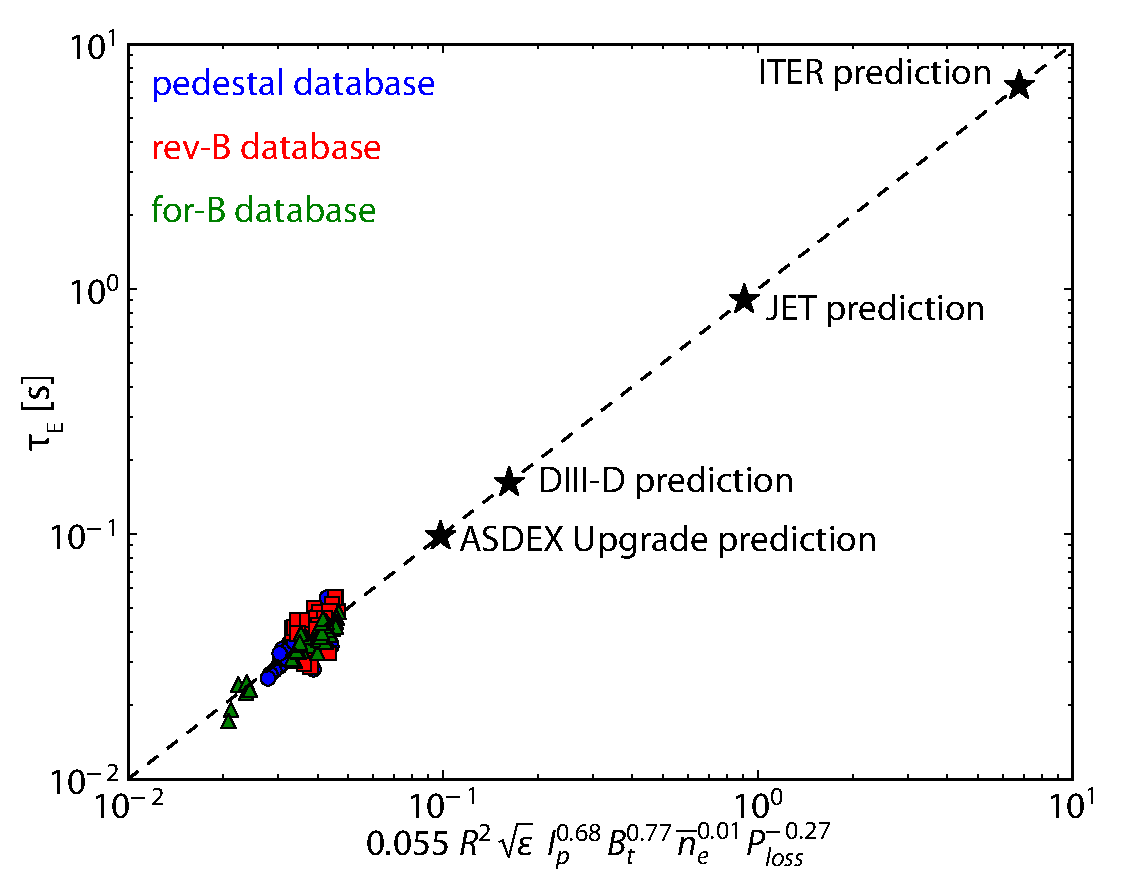
\includegraphics[width=100mm]{graphics/IModePedestal/tauE_6_Ploss_extrap.pdf}}
\end{figure}

\nicesectionending

\section{Conclusions}\label{sec:imode_ped_conclusions}

\nicechapterending

\bibliographystyle{../plainurl}
\bibliography{../references}